\documentclass[varwidth=true, border=2pt]{standalone}
\usepackage{tkz-euclide}

\begin{document}
\usetkzobj{all}
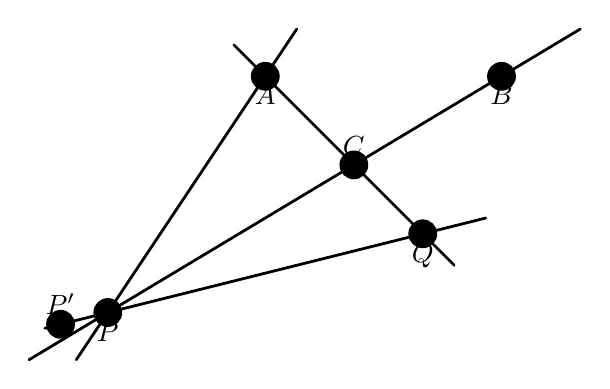
\begin{tikzpicture}
    \tkzSetUpPoint[shape=circle,size=10,color=black,fill=black]
    \tkzSetUpLine[line width=1]
    \tkzDefPoints{0/0/P, 4/1/Q, 2/3/A, 5/3/B, -0.6/-0.15/Pstrich}
    \tkzInterLL(P,B)(A,Q) \tkzGetPoint{C}
    \tkzDrawPoints(P,Q,A,B,C,Pstrich)

    \tkzDrawLine(P,Q)
    \tkzDrawLine(P,A)
    \tkzDrawLine(A,Q)
    \tkzDrawLine(P,B)

    \tkzLabelPoint[below](P){$P$}
    \tkzLabelPoint[above](Pstrich){$P'$}
    \tkzLabelPoint[below](Q){$Q$}
    \tkzLabelPoint[below](A){$A$}
    \tkzLabelPoint[below](B){$B$}
    \tkzLabelPoint[above](C){$C$}
\end{tikzpicture}
\end{document}
